\documentclass[11pt,a4paper]{article}

\usepackage[utf8]{inputenc}
\usepackage[T1]{fontenc}
\usepackage[english]{babel}
\usepackage[a4paper,margin=2.4cm]{geometry}

\usepackage{amsmath, amssymb, amsthm}
\usepackage{mathtools}
\usepackage{stmaryrd}
\usepackage{booktabs}
\usepackage{tabularx}
\usepackage{array}
\usepackage{caption}
\usepackage{subcaption}
\usepackage{float}
\usepackage{enumitem}
\usepackage{microtype}
\usepackage{xcolor}
\usepackage{listings}
\usepackage{fancyhdr}
\usepackage{titlesec}
\usepackage{graphicx}
\usepackage{tikz}
\usetikzlibrary{positioning, arrows.meta, fit, backgrounds, calc, shapes.geometric}
\usepackage[hidelinks]{hyperref}

%  ---  Palette shared with the companion reports  ---
\definecolor{ink}{RGB}{26,30,36}
\definecolor{slate}{RGB}{92,101,112}
\definecolor{mist}{RGB}{233,235,238}
\definecolor{rulegrey}{RGB}{188,194,201}
\definecolor{steel}{RGB}{47,72,102}
\definecolor{steellight}{RGB}{124,146,172}
\definecolor{signal}{RGB}{160,32,45}
\definecolor{southc}{RGB}{51,115,204}
\definecolor{northc}{RGB}{230,128,38}
\definecolor{knows}{RGB}{26,140,70}

\hypersetup{
    colorlinks=true,
    linkcolor=steel,
    citecolor=steel,
    urlcolor=steel,
    pdftitle={The Coordinated Attack among Many Robots},
    pdfauthor={Haniel Ulises},
}

\color{ink}

\setlength{\headheight}{22pt}
\pagestyle{fancy}
\fancyhf{}
\fancyhead[L]{\small\textcolor{slate}{\itshape The Coordinated Attack among Many Robots}}
\fancyhead[R]{\small\textcolor{slate}{\thepage}}
\renewcommand{\headrulewidth}{0.4pt}
\renewcommand{\headrule}{\hbox to\headwidth{\color{rulegrey}\leaders\hrule height \headrulewidth\hfill}}

\titleformat{\section}{\normalfont\large\bfseries\color{ink}}{\thesection}{0.7em}{}
\titleformat{\subsection}{\normalfont\normalsize\bfseries\color{ink}}{\thesubsection}{0.7em}{}
\titleformat{\paragraph}[runin]{\normalfont\bfseries\color{slate}}{}{0em}{}[.]

\captionsetup{font=small, labelfont={bf,color=slate}, textfont=footnotesize}

\theoremstyle{definition}
\newtheorem{definition}{Definition}
\newtheorem{proposition}{Proposition}
\newtheorem{lemma}{Lemma}
\newtheorem{corollary}{Corollary}
\newtheorem{fact}{Fact}
\newtheorem{remark}{Remark}

\lstdefinestyle{sys}{
    backgroundcolor=\color{mist},
    basicstyle=\ttfamily\scriptsize\color{ink},
    keywordstyle=\color{steel}\bfseries,
    commentstyle=\color{slate}\itshape,
    stringstyle=\color{slate},
    morecomment=[l]{;},
    morekeywords={:types,:predicates,:objects,:agents,:goal,:init,:event,:action,:action-type,:observability-conditions,:precondition,:effects,:events,:relations,:designated,:conditions,:observability-types},
    frame=single,
    rulecolor=\color{rulegrey},
    framesep=5pt,
    xleftmargin=6pt,
    xrightmargin=0pt,
    breaklines=true,
    showstringspaces=false,
    columns=fullflexible,
    captionpos=b,
}
\lstset{style=sys}

%  ---  Notation  ---
\newcommand{\Ag}{\mathcal{A}}
\newcommand{\Mod}{\mathcal{M}}
\newcommand{\Ev}{\mathcal{E}}
\newcommand{\prd}{\otimes}
\newcommand{\Kop}[1]{K_{#1}}
\newcommand{\Eop}[1]{E_{#1}}
\newcommand{\Cop}[1]{C_{#1}}
\newcommand{\Kw}[1]{\mathit{Kw}_{#1}}
\newcommand{\code}[1]{\texttt{\small #1}}
\newcommand{\ag}[1]{\mathit{#1}}
\newcommand{\job}{\mathit{job}}
\newcommand{\pre}{\mathit{pre}}
\newcommand{\post}{\mathit{post}}
\newcommand{\dist}{\mathrm{dist}}
\newcommand{\depth}{\mathrm{depth}}
\newcommand{\atview}{\mathit{at\text{-}view}}
\newcommand{\sem}[1]{\llbracket #1 \rrbracket}

\newcommand{\sent}{\mathit{sent}}

\begin{document}

\begin{titlepage}
\centering
\vspace*{2.4cm}
{\color{rulegrey}\rule{\textwidth}{0.8pt}}\\[0.9cm]
{\LARGE\bfseries The Coordinated Attack among Many Robots\par}
\vspace{0.5cm}
{\large\color{slate} Bystanders to a Lossy Message, the Cost of Each Level\\
of Mutual Knowledge, and Four Robots on the Floor\par}
\vspace{0.7cm}
{\color{rulegrey}\rule{\textwidth}{0.8pt}}\\[1.4cm]

{\large Haniel Ulises\par}
\vspace{0.3cm}
{\color{slate} Epistemic Robotics}\\
\vspace{0.15cm}
{\color{slate}\today}

\vfill
{\color{slate}\small
The companion report states common knowledge of a stand as the precondition of
a joint lift by two robots, proves that a lossy radio cannot supply it, and
executes the policy a beacon makes possible. This report writes the same
domain for $N$ robots and $m$ message levels. Every robot takes a share of the
load, so the lift requires common knowledge over all $N$, and a message at
level $\ell$ states that its sender knows that everyone knows, $\ell-1$ times
over, which stand the order names.

\vspace{0.6em}
With more than two robots a message has bystanders, robots that neither send
nor receive it. We give them an observability type of their own, relating the
three events of the message to one another, and show that the product update
with such a message still preserves $\mathrm{S5}$ and still adds at most one
level of mutual knowledge, so that no finite exchange yields common knowledge,
for any number of robots. A signal observed from viewpoints that are common
knowledge yields it over all $N$ in one update. The planner returns the beacon
policy, of depth $N+3$, for up to ten robots, and its proofs on the radio floor
run out of budget from three robots and two levels. Among $N$ robots it found
$E^k$ to cost $k(N-1)$ messages in every cell it settled, and showed in the
others that fewer do not suffice: a message says more than its content,
because a robot that knows the stand can only have learnt it from one that
knew first. Four robots were executed in Gazebo through ePlanSys. Over the
radio, six delivered messages reached $E^2$ and the executor refused the lift;
with the beacon, one signal gave common knowledge over all four, and the four
lifted together, arrivals 0.10\,s apart.}
\vspace{1.2cm}
\end{titlepage}

\tableofcontents
\newpage

%  ======================================================================
\section{Scope}
\label{sec:scope}

The companion report~\cite{ulises2026ca} concerns two robots, south and north,
which must lift one load together after one of them has read which of two
stands it is on. Its results are stated for the group of the two, and two of
its arguments use that the group has two members: the proof that a message adds
at most one level of mutual knowledge distinguishes only the sender and the
receiver, and the floor has one viewpoint at each mouth of the bay. This report
removes the restriction. The domain is written for any number $N$ of robots,
all of which take a share of the load, and for any number $m$ of message
levels, and the question is which of the companion report's results survive,
and at what cost to the planner.

Four claims are advanced.

\begin{enumerate}[leftmargin=1.4em, itemsep=2pt]
  \item When a robot that neither sends nor receives a message relates its
        three events, the lossy message preserves $\mathrm{S5}$ and adds at
        most one level of mutual knowledge in a group of any size
        (Propositions~\ref{prop:s5} and~\ref{prop:onelevel}). On the radio
        floor no policy exists, for any number of robots or messages
        (Corollary~\ref{cor:radio}).
  \item One signal from viewpoints that are common knowledge yields common
        knowledge over all $N$ (Proposition~\ref{prop:public}), and the
        planner returns a policy of depth $N + 3$ for every $N$ up to ten, each
        of whose leaves the product update confirms.
  \item Among $N$ robots the fewest messages that reach $E^k$ were $k(N-1)$ in
        every cell the planner settled, and at least $k(N-1)$ in the others.
        The protocols it finds use what a message implies beyond its content.
  \item Four robots executed both floors in simulation, with the precondition
        checked by the executor against the model, and the depth of mutual
        knowledge computed from the live model after each message agreed with
        the offline replay.
\end{enumerate}

Four bounds are stated at the outset. The search settles the radio floor only
for two robots up to five levels and for three robots at one level; beyond
that it ran out of budget, and the floor is settled by
Corollary~\ref{cor:radio} and not by search. The count $k(N-1)$ is a pattern
over the cells, minimal in each within the family of messages the domain
defines, and is not proved in general. The floor has places for four robots,
so the runs stop at four, while the planner's tables go to ten. And the
positions domain of the companion report, in which a move is witnessed only by
the robot that makes it, is written for a pair and was not extended. The
bounds of the companion report also hold here: every message in the runs is
delivered, the lift is drawn by moving the load in the simulator, and the
positions of the robots are common knowledge because the move to a viewpoint is
public.

%  ======================================================================
\section{Preliminaries}
\label{sec:prelim}

The definitions are those of the companion report, restated in the form this
report uses.

\begin{definition}[Epistemic model]
Let $\Ag$ be a finite set of agents and $P$ a finite set of atoms. An
\emph{epistemic model} is $\Mod = (W, R, V, W_d)$ with $W$ a finite set of
worlds, $R : \Ag \to 2^{W\times W}$, $V : W \to 2^P$, and
$\emptyset \neq W_d \subseteq W$ the designated worlds. $\Mod$ is
$\mathrm{S5}$ when every $R_a$ is an equivalence. A formula holds at $\Mod$ when
it holds at every designated world.
\end{definition}

\begin{definition}[Group modalities]
For $G \subseteq \Ag$ let $R_G = \bigcup_{a\in G} R_a$ and $R_G^+$ its
transitive closure. $\Mod, w \models \Eop{G}\varphi$ iff $\varphi$ holds at
every $v$ with $w R_G v$; $\Eop{G}^{k+1}\varphi = \Eop{G}\Eop{G}^{k}\varphi$
and $\Eop{G}^0\varphi = \varphi$; and $\Mod, w \models \Cop{G}\varphi$ iff
$\varphi$ holds at every $v$ with $w R_G^+ v$.
\end{definition}

\begin{definition}[Distance and depth]
\label{def:depth}
For $\Mod \models \varphi$, $\dist_\Mod(\varphi)$ is the least $m$ such that
some designated world reaches, by an $R_G$-path of length $m$, a world where
$\varphi$ fails, and $\infty$ if there is none. The \emph{depth} of $\varphi$
is $\depth_\Mod(\varphi) = \dist_\Mod(\varphi) - 1$.
\end{definition}

\begin{lemma}
\label{lem:depth}
If $\Mod$ is $\mathrm{S5}$ and $\Mod \models \varphi$, then for $k \geq 1$,
$\Mod \models \Eop{G}^k\varphi$ iff $k \leq \depth_\Mod(\varphi)$, and
$\Mod \models \Cop{G}\varphi$ iff $\dist_\Mod(\varphi) = \infty$.
\end{lemma}

\begin{proof}
$\Eop{G}^k\varphi$ holds at $w$ iff $\varphi$ holds at every world reached from
$w$ by an $R_G$-path of length exactly $k$. Each $R_a$ is reflexive, so the
worlds reached in exactly $k$ steps are those reached in at most $k$, and
$\Eop{G}^k\varphi$ fails at a designated world iff a counterexample lies within
distance $k$ of it. The case of $\Cop{G}$ is the union over $k$.
\end{proof}

\begin{definition}[Event model and product update]
An \emph{event model} is $\Ev = (E, T, Q, \pre, \post, E_d)$ with events $E$,
observability types $T$, $Q : T \to 2^{E\times E}$, preconditions, postconditions
and designated events $E_d$. Each agent $a$ has a type $\tau_a$ for the whole
model, the type whose observability condition holds at the designated worlds.
The product update $\Mod \prd \Ev$ has worlds
$W' = \{(w,e) : \Mod, w \models \pre(e)\}$, relations
$(w,e)\, R'_a\, (v,f)$ iff $w R_a v$ and $(e,f) \in Q(\tau_a)$, valuation by the
postconditions, and designated worlds $W'_d = (W_d \times E_d) \cap W'$. $\Ev$
is \emph{applicable} in $\Mod$ when every designated world has a designated
event whose precondition holds there.
\end{definition}

\begin{definition}[Lossy message]
\label{def:lossy}
For agents $i \neq j$, a formula $\pi$ and an atom $p$, $L(i,j,\pi,p)$ has
events $d$ (delivered), $l$ (lost) and $n$ (never sent),
$\pre(d) = \pre(l) = \pi$, $\pre(n) = \top$, $\post(d) = \post(l) =
\{p \mapsto \top\}$, $\post(n)$ trivial, $E_d = \{d\}$, and types
\[
  Q(\mathrm{Sender}) = \{d,l\}^2 \cup \{(n,n)\},\qquad
  Q(\mathrm{Receiver}) = \{(d,d)\} \cup \{l,n\}^2,
\]
with $\tau_i = \mathrm{Sender}$ and $\tau_j = \mathrm{Receiver}$.
\end{definition}

\noindent
The sender knows it sent and cannot tell whether the message arrived; the
receiver knows whether something arrived and, when nothing did, cannot tell a
loss from silence. With two robots every agent is the sender or the receiver.
With more, the definition leaves the other robots without a type.

%  ======================================================================
\section{The domain for $N$ robots}
\label{sec:domain}

The generator \code{tools/scaled.py} writes the domain for $N$ robots and $m$
message levels, and the launch file runs it with \code{robots:=} and
\code{messages:=}. The robots are south, north, south2, north2, and so on,
alternately on the storage and the dispatch floor; $G$ is the set of all of
them, and south reads the order. Every robot takes a share of the load, so
$\mathit{lift}(s)$ requires $\Cop{G}\job(s)$. A message at level $\ell$ from
$i$ to $j$ is the lossy message $L(i,j,\pi,p)$ with
\[
  \pi = \Kop{i}\Eop{G}^{\ell-1}\job(s) \wedge \neg p,
  \qquad p = \sent_\ell(i,j):
\]
the sender knows that everyone knows, $\ell-1$ times over, which stand the
order names, and each level goes from each sender to each receiver at most
once. Level 1 is $\mathit{tell}$, level 2 $\mathit{ack}$, level 3
$\mathit{ack2}$, and so on. Table~\ref{tab:actions} gives the actions.

\begin{table}[H]
\centering\small
\caption{The actions of the domain for $N$ robots and $m$ levels.}
\label{tab:actions}
\begin{tabularx}{\textwidth}{@{}>{\raggedright\arraybackslash}p{3.3cm} >{\raggedright\arraybackslash}p{2.5cm} >{\raggedright\arraybackslash}X >{\raggedright\arraybackslash}p{3.1cm}@{}}
\toprule
action & type & events & observers \\
\midrule
$\mathit{read\text{-}order}(i, s)$ & semi-private sensing & $e_h$: $\job(s)$; $e_e$: $\neg\job(s)$; both with $\neg\atview(i) \wedge \neg\Kw{i}\job(s)$ & $i$ fully, every other robot partially \\
$\mathit{tell}$, $\mathit{ack}$, \dots\ $(i,j,s)$, level $\ell \leq m$ & lossy message & $d$, $l$: $\Kop{i}\Eop{G}^{\ell-1}\job(s) \wedge \neg\sent_\ell(i,j)$, post $\sent_\ell(i,j)$; $n$: $\top$ & $i$ sender, $j$ receiver, every other robot a bystander \\
$\mathit{go\text{-}view}(i)$ & public ontic & $\mathit{beacon} \wedge \neg\atview(i)$, post $\atview(i)$ & everyone \\
$\mathit{signal}(i, s)$ & conditional announcement & $\sigma$: $\atview(i) \wedge \Kop{i}\job(s)$; $n$: $\top$ & at a viewpoint fully, elsewhere obliviously \\
$\mathit{lift}(s)$ & public ontic & $\job(s) \wedge \Cop{G}\job(s)$, post $\mathit{lifted}$ & everyone \\
\bottomrule
\end{tabularx}
\end{table}

\paragraph{Two robots} With $N = 2$ the content of each message is the
companion report's. $\Eop{G}$ is then $\Kop{\ag{south}} \wedge
\Kop{\ag{north}}$, and $\Kop{i}\Eop{G}^{\ell-1}\job(s)$ is equivalent in
$\mathrm{S5}$ to the alternating $\Kop{i}\Kop{j}\Kop{i}\cdots\job(s)$ with
$\ell$ operators, the conjuncts that repeat an agent collapsing by
introspection. The log differs. The companion domain lets each level go out
once in all, and this one once per sender and receiver, so that at $N = 2$ it
admits each message and its mirror image. Its beacon floor has the policy of
depth five, found in 137 expansions where the companion domain takes 115; its
radio floor is exhausted at depth 9 with 2\,224 expansions, where the
companion's is exhausted at depth 5 with 34.

%  ======================================================================
\section{Robots that neither send nor receive}
\label{sec:bystanders}

\begin{definition}[Bystander]
\label{def:bystander}
In a lossy message $L(i,j,\pi,p)$ among a group $G \supseteq \{i,j\}$, every
$b \in G \setminus \{i,j\}$ has $\tau_b = \mathrm{Bystander}$, with
$Q(\mathrm{Bystander}) = E \times E$.
\end{definition}

A robot that does not hear the radio cannot tell a delivery from a loss or from
silence. The library's Oblivious type, which maps every event onto $n$, would
not serve. Since $d$ and $l$ set the sender's log, an oblivious bystander at
$(w,d)$ would consider possible only worlds at which $p$ fails, so that $R'_b$
would not be reflexive: the bystander would believe that no message went out
when one did, and the model would leave $\mathrm{S5}$. The type is added to
\code{epddl/lossy.epddl} (Listing~\ref{lst:lossy}). The companion report's
floors never assign it, and their grounded tasks are unchanged apart from the
added relation.

\begin{lstlisting}[caption={The action type, in \code{epddl/lossy.epddl}, with the bystander type.}, label={lst:lossy}]
(:action-type lossy-message
  :events     (?del ?lost ?nil)
  :observability-types (Sender Receiver Bystander Oblivious)
  :relations  (Sender    (:and (?del ?del) (?del ?lost) (?lost ?del) (?lost ?lost) (?nil ?nil))
               Receiver  (:and (?del ?del) (?lost ?lost) (?lost ?nil) (?nil ?lost) (?nil ?nil))
               Bystander (:forall (?e ?f - event) (?e ?f))
               Oblivious (:forall (?e - event) (?e ?nil)) )
  :designated (?del)
  :conditions (?nil (:trivial-event)))
\end{lstlisting}

\begin{figure}[H]
\centering
\begin{tikzpicture}[
  ev/.style={draw, rounded corners=3pt, minimum width=1.9cm, minimum height=0.75cm, fill=mist, font=\ttfamily\small},
  des/.style={ev, draw=signal, line width=1.3pt},
  lab/.style={font=\scriptsize, text=slate}]
\node[des] (d) at (0,0) {d};
\node[ev] (l) at (4,0) {l};
\node[ev] (n) at (8,0) {n};
\draw[southc, line width=1.4pt] (d) -- node[above, font=\small] {$i$} (l);
\draw[northc, line width=1.4pt] (l) -- node[above, font=\small] {$j$} (n);
\draw[knows, line width=1.2pt, dashed] (d.south) .. controls +(0,-1.3) and +(0,-1.3) .. node[below, font=\small] {$b$} (n.south);
\node[lab, above=0.45cm of d] {delivered, designated};
\node[lab, above=0.45cm of l] {sent and lost};
\node[lab, above=0.45cm of n] {never sent};
\end{tikzpicture}
\caption{The lossy message among three or more robots. Reflexive edges are
omitted. The sender $i$ relates $d$ and $l$, the receiver $j$ relates $l$ and
$n$, and a bystander $b$ relates all three events; only the edge it adds between
$d$ and $n$ is drawn.}
\label{fig:lossy}
\end{figure}

\begin{proposition}[$\mathrm{S5}$ is preserved]
\label{prop:s5}
If $\Mod$ is $\mathrm{S5}$, so is $\Mod \prd L(i,j,\pi,p)$, with any number of
bystanders.
\end{proposition}

\begin{proof}
$R'_a$ is the restriction to $W'$ of the relation
$\{((w,e),(v,f)) : w R_a v,\ (e,f) \in Q(\tau_a)\}$ on $W \times E$. For each of
the three types $Q(\tau_a)$ is an equivalence, $E \times E$ among them, so
this is a product of equivalences, and its restriction to a subset is an
equivalence.
\end{proof}

\begin{proposition}[At most one level per message, in any group]
\label{prop:onelevel}
Let $G$ be a finite group with $i \neq j$ in $G$ and every other member a
bystander of $L = L(i,j,\pi,p)$. Let $\Mod$ be $\mathrm{S5}$ with
$\Mod \models \varphi$, let $\varphi$ not mention $p$, and let $\pi$ be such that
$\Mod, w \models \pi$ and $w R_i v$ imply $\Mod, v \models \pi$. If $L$ is
applicable in $\Mod$, then
\[
  \dist_{\Mod \prd L}(\varphi) \;\leq\; \dist_\Mod(\varphi) + 1 .
\]
\end{proposition}

\begin{proof}
If $\dist_\Mod(\varphi) = \infty$ there is nothing to show. Otherwise let
$w \in W_d$ and $w = v_0 \xrightarrow{a_1} v_1 \xrightarrow{a_2} \cdots
\xrightarrow{a_m} v_m$ be an $R_G$-path with $m = \dist_\Mod(\varphi) \geq 1$ and
$\Mod, v_m \not\models \varphi$. Since $L$ is applicable, $(w,d) \in W'_d$.
Since $\pre(n) = \top$, $(v,n) \in W'$ for every $v \in W$, and since
$(n,n) \in Q(\tau)$ for all three types, $v R_a u$ implies
$(v,n) R'_a (u,n)$ for every $a \in G$: the $n$-copies form a copy of $\Mod$.
As $\post(n)$ is trivial and $\varphi$ does not mention $p$, $(v_m, n)$
falsifies $\varphi$. Three cases.

\emph{$a_1 = j$.} $(v_0,l) \in W'$ since $\pre(l) = \pre(d)$. Then
$(v_0,d) \mathrel{R'_i} (v_0,l)$ by reflexivity and $(d,l) \in Q(\mathrm{Sender})$,
and $(v_0,l) \mathrel{R'_j} (v_1,n)$ by $v_0 R_j v_1$ and
$(l,n) \in Q(\mathrm{Receiver})$: two steps.

\emph{$a_1 = i$.} $\Mod, v_1 \models \pi$ by the hypothesis on $\pi$, so
$(v_1,l) \in W'$. Then $(v_0,d) \mathrel{R'_i} (v_1,l)$ by $v_0 R_i v_1$ and
$(d,l) \in Q(\mathrm{Sender})$, and $(v_1,l) \mathrel{R'_j} (v_1,n)$ by
reflexivity and $(l,n) \in Q(\mathrm{Receiver})$: two steps.

\emph{$a_1 = b$, a bystander.} $(v_0,d) \mathrel{R'_b} (v_1,n)$ by
$v_0 R_b v_1$ and $(d,n) \in Q(\mathrm{Bystander})$: one step.

In each case at most two steps reach $(v_1, n)$, and $m-1$ further steps along
the $n$-copy of the path reach $(v_m,n)$: a path of length at most $m+1$ from a
designated world to a counterexample.
\end{proof}

\noindent
The first two cases are the companion report's proof. The third is the only
one the bystanders add, and it shortens the path: a bystander's edge from the
delivered event to the event in which nothing was sent is an edge of the
product the two-robot proof had to build in two steps. The proof does not use
that $d$ is the event that occurred, so the bound holds whether the message is
delivered or lost.

\begin{corollary}[No finite exchange yields common knowledge]
\label{cor:radio}
Under the hypotheses of Proposition~\ref{prop:onelevel}, if
$\Mod \not\models \Cop{G}\varphi$ then
$\Mod \prd L_1 \prd \cdots \prd L_k \not\models \Cop{G}\varphi$ for every finite
sequence of lossy messages. On the radio floor, for every $N \geq 2$ and every
$m$, no sequence of applicable actions makes $\mathit{lift}(s)$ applicable for
either $s$, and no policy for $\mathit{lifted}$ exists.
\end{corollary}

\begin{proof}
The first part is Propositions~\ref{prop:s5} and~\ref{prop:onelevel} and
Lemma~\ref{lem:depth}, by induction on $k$. On the radio floor
$\mathit{beacon}$ is false, so $\mathit{go\text{-}view}$ and $\mathit{signal}$
are never applicable. A message requires $\Kop{\ag{south}}\job(s)$ or a
statement over it, which fails until the order is read, and
$\mathit{read\text{-}order}$ is applicable at most once. Every execution is
therefore the reading followed by lossy messages. Before the reading,
$\job(s)$ fails at one of the two designated worlds. After it, on the branch
where the order names $s$, $\job(s)$ holds at the designated world, and every
robot but south, observing the reading partially, relates it to the copy of the
other world: $\dist(\job(s)) = 1$. The hypothesis on $\pi$ holds for every
message. $\Kop{i}\Eop{G}^{\ell-1}\job(s)$ is preserved along $R_i$ by positive
introspection, and $\sent_\ell(i,j)$ is set only by a message that $i$ sends,
whose Sender type separates $n$ from $d$ and $l$, so that its value is the same
at all worlds $R_i$ relates. By the first part the distance stays finite after
every message, and by Lemma~\ref{lem:depth} $\Cop{G}\job(s)$ never holds.
\end{proof}

%  ======================================================================
\section{The beacon for $N$ robots}
\label{sec:beacon}

\begin{proposition}[A signal seen from common viewpoints]
\label{prop:public}
Let $\Mod$ be $\mathrm{S5}$ with $\atview(a)$ true at every world of $\Mod$ for
every $a \in G$. If $S = S(i,\Kop{i}\chi)$ is applicable in $\Mod$, then
$\Mod \prd S \models \Cop{G}\chi$, whatever the size of $G$.
\end{proposition}

\begin{proof}
Every type is Fully, so $(w,e) R'_a (v,f)$ implies $e = f$, and every world
$R_G^+$-reachable from a designated $(w,\sigma)$ is of the form $(v,\sigma)$.
$(v,\sigma) \in W'$ requires $\Mod, v \models \Kop{i}\chi$, which gives
$\Mod, v \models \chi$; as $\post(\sigma)$ is trivial, $\chi$ holds at every
reachable world.
\end{proof}

\noindent
As in the companion report, $\atview$ is set by the public
$\mathit{go\text{-}view}$, so once every robot has moved its position is common
knowledge, and the hypothesis holds. The policy the planner returns is the
companion report's with a viewpoint for every robot: each robot but the reader
goes to its viewpoint, the order is read, the reader goes to its viewpoint and
signals, and the robots lift. Its depth is $N + 3$, and it has two leaves, one
per stand. The product update of the trace tool replays every policy found and
reports $\Cop{G}\job(s)$ at both leaves, for every $N$ up to ten.

%  ======================================================================
\section{Planning results}
\label{sec:planning}

Tables~\ref{tab:scale-beacon} and~\ref{tab:scale-radio} are written by
\code{tools/scaling.py}: plank grounds each cell, and Aletheia solves it at one
thread, once with AO$^*$ and once replanning over the all-outcomes
determinization, each with a budget of 300\,s. AO$^*$ deepens one action at a
time and checks its budget inside each iteration. An entry \emph{cut off at
depth $d$} means that the budget ran out in the iteration at depth $d$, so that
no policy of smaller depth exists. The beacon floor is written with four
message levels throughout, which it never uses.

\begin{table}[H]
\centering\small
\caption{The beacon floor with $N$ robots: the depth of the policy, the
expansions and the time. Every policy found has two leaves, and the trace tool
reports $\Cop{G}\job(s)$ at both. Atom counts are plank's, and include the log
atoms $\sent_\ell(i,i)$, which no action sets.}
\label{tab:scale-beacon}
\begin{tabular}{@{}r r r l l@{}}
\toprule
$N$ & atoms & actions & AO$^*$ & replanning \\
\midrule
2 & 24 & 28 & depth 5, 137, 0.0\,s & depth 5, 8, 0.0\,s \\
3 & 46 & 65 & depth 6, 868, 0.2\,s & depth 6, 11, 0.0\,s \\
4 & 76 & 118 & depth 7, 8\,038, 4.6\,s & depth 7, 14, 0.0\,s \\
5 & 114 & 187 & depth 8, 108\,298, 112.3\,s & depth 8, 17, 0.0\,s \\
6 & 160 & 272 & cut off at depth 8, 165\,772 & depth 9, 20, 0.1\,s \\
7 & 214 & 373 & cut off at depth 7, 99\,175 & depth 10, 23, 0.1\,s \\
8 & 276 & 490 & cut off at depth 7, 84\,110 & depth 11, 26, 0.2\,s \\
9 & 346 & 623 & cut off at depth 7, 78\,032 & depth 12, 29, 0.4\,s \\
10 & 424 & 772 & cut off at depth 7, 68\,467 & depth 13, 32, 0.7\,s \\
\bottomrule
\end{tabular}
\end{table}

\noindent
AO$^*$ pays about a factor of ten in expansions for each robot. At six robots
its budget runs out one iteration short of the policy, and from seven on it
does not reach depth eight. Replanning finds the same policy in $3N + 2$
expansions, ten robots in under a second.

\begin{table}[H]
\centering\small
\caption{The radio floor with $N$ robots and $m$ levels. There is no policy;
a cell gives how the search ended, the expansions and the time.}
\label{tab:scale-radio}
\begin{tabular}{@{}r r r r l l@{}}
\toprule
$N$ & $m$ & atoms & actions & AO$^*$ & replanning \\
\midrule
2 & 1 & 12 & 16 & exhausted at depth 3, 14, 0.0\,s & refuted, 5, 0.0\,s \\
2 & 2 & 16 & 20 & exhausted at depth 5, 52, 0.0\,s & refuted, 15, 0.0\,s \\
2 & 3 & 20 & 24 & exhausted at depth 7, 282, 0.1\,s & refuted, 81, 0.0\,s \\
2 & 4 & 24 & 28 & exhausted at depth 9, 2\,224, 1.7\,s & refuted, 563, 0.8\,s \\
2 & 5 & 28 & 32 & exhausted at depth 11, 18\,990, 45.9\,s & refuted, 3\,989, 18.4\,s \\
2 & 6 & 32 & 36 & cut off at depth 12, 89\,529 & cut off, 16\,350 \\
3 & 1 & 19 & 29 & exhausted at depth 7, 294, 0.1\,s & refuted, 67, 0.1\,s \\
3 & 2 & 28 & 41 & cut off at depth 10, 36\,517 & cut off, 353 \\
3 & 3 & 37 & 53 & cut off at depth 10, 74\,958 & cut off, 26 \\
4 & 1 & 28 & 46 & cut off at depth 9, 20\,500 & cut off, 435 \\
4 & 2 & 44 & 70 & cut off at depth 9, 48\,601 & cut off, 17 \\
5 & 1 & 39 & 67 & cut off at depth 8, 37\,629 & cut off, 15 \\
\bottomrule
\end{tabular}
\end{table}

\noindent
On the radio floor what is measured is the price of proving that no policy
exists. AO$^*$ proves it by exhausting the space. Replanning proves it by
refuting the determinization, which is sound for unsolvability, since any
branch of a policy of the task is a plan of its determinization. At two robots
both proofs finish up to five levels, and each level costs AO$^*$ a factor that
rises to about eight. A third robot leaves one level within reach, and a fourth
none: the space is every order in which up to $N(N-1)m$ messages can go out,
and it outgrows the search long before the robots fill the floor. Where a
search was cut off, nothing is claimed from it; that none of these floors has a
policy is Corollary~\ref{cor:radio}.

\paragraph{How the counts were taken} Aletheia, at commit \code{314bc29},
prints a search's expansions only when it finds a policy. The counts for
searches that ended without one were taken with a build that also prints them
there and changes nothing else; on the four floors of the companion report it
returns the installed planner's results, expansion for expansion. Replanning
overran its budget on the larger radio floors, in a step that does not check
the clock: by 40\,\% at five robots, and in an earlier run, at four robots and
two levels, to 673\,s before it was stopped. The harness kills a run at one and
a half times its budget and thirty seconds more. Eight searches ran at once,
alongside four processes of the search of Section~\ref{sec:ladder}, on sixteen
hardware threads, so the expansions are the measure and the times are orders of
magnitude.

%  ======================================================================
\section{What each level costs}
\label{sec:ladder}

\code{tools/ladder.py} gives the planner the radio floor with the goal
$\Eop{G}^k\job(s)$ in place of $\mathit{lifted}$. AO$^*$ deepens one action at
a time, so the first policy it finds has the fewest messages that reach
$\Eop{G}^k$, among the messages of the domain. The trace tool's product update
then replays the policy; it must agree on the depth after every message, and
find at the end that $\Cop{G}\job(s)$ fails and $\mathit{lift}$ is not
applicable.

\begin{table}[H]
\centering\small
\caption{The fewest messages that reach $\Eop{G}^k\job(s)$ among $N$ robots.
An entry $\geq c$ is a search cut off in the iteration that would hold $c$
messages: no protocol of fewer exists, and none of $c$ was found. The budget was
600\,s, and an hour for four robots and $\Eop{G}^3$. Blank cells were not run.}
\label{tab:ladder}
\begin{tabular}{@{}r r r r r r@{}}
\toprule
$N$ & $\Eop{G}^1$ & $\Eop{G}^2$ & $\Eop{G}^3$ & $\Eop{G}^4$ & $\Eop{G}^5$ \\
\midrule
2 & 1 & 2 & 3 & 4 & 5 \\
3 & 2 & 4 & 6 & 8 & $\geq 10$ \\
4 & 3 & 6 & $\geq 9$ & & \\
5 & 4 & $\geq 8$ & & & \\
\bottomrule
\end{tabular}
\end{table}

\noindent
Wherever the search finished, $\Eop{G}^k$ cost $k(N-1)$ messages, and wherever
it was cut off it had shown that fewer do not suffice. For two robots this is
the bound of Proposition~\ref{prop:onelevel}, attained. For more, the count is
a pattern over the cells, minimal in each within this family of messages, and
it is not proved in general.

It is fewer messages than their levels suggest. A robot that knows where the
load is can only have learnt it from one that knew first, and the messages of
the history are the only ones that can have occurred, so a message says more
than its content: when north tells south2 $\Kop{\ag{north}}\job(s)$, south2
also learns that south knew, since north could have heard it from no one else.
The protocols the planner finds use this. With three robots they relay along a
line, south, north, south2, and back. With four, $\Eop{G}^2$ is a relay out to
north2 and a broadcast back from it (Table~\ref{tab:protocol}), and this is the
protocol the mission runs on the four-robot radio floor.

\begin{table}[H]
\centering\small
\caption{The protocol for $\Eop{G}^2$ among four robots, on the branch where
the order names $s_1$. Worlds are those of the model the epistemic state kept
during the run; the offline replay gives the same depths and counts.}
\label{tab:protocol}
\begin{tabular}{@{}l r l@{}}
\toprule
action & $|W|$ & depth of $\job(s_1)$ \\
\midrule
$\mathit{read\text{-}order}(\ag{south}, s_1) \to e_h$ & 2 & $E^0$ \\
$\mathit{tell}(\ag{south}, \ag{north}, s_1)$ & 4 & $E^0$ \\
$\mathit{tell}(\ag{north}, \ag{south2}, s_1)$ & 6 & $E^0$ \\
$\mathit{tell}(\ag{south2}, \ag{north2}, s_1)$ & 8 & $E^1$ \\
$\mathit{ack}(\ag{north2}, \ag{north}, s_1)$ & 10 & $E^1$ \\
$\mathit{ack}(\ag{north2}, \ag{south2}, s_1)$ & 16 & $E^1$ \\
$\mathit{ack}(\ag{north2}, \ag{south}, s_1)$ & 34 & $E^2$ \\
$\mathit{lift}(s_1)$ & \multicolumn{2}{l}{not applicable: $\Cop{G}\job(s_1)$ fails} \\
\bottomrule
\end{tabular}
\end{table}

\noindent
The third message is the first to raise the depth. After it north2 knows the
stand, and also that south2 knew it, that north did, and that south did, since
each could have learnt it only from the one before; that is $\Eop{G}^1$, and
each robot knows it of every other only once north2's acknowledgements have
gone back down the line.

%  ======================================================================
\section{The floor with four robots}
\label{sec:floor}

The floor is the companion report's: the pass-through floor, a racking block
across a $30 \times 50$\,m hall, the loads in bays $t_1$ and $t_3$ as the
stands $s_1$ and $s_2$, and the beacon in the open bay $t_2$
(Figure~\ref{fig:floor}). south2 starts at the east end of the storage floor's
southern aisle and north2 at the west end of the dispatch floor's northern
aisle. Each mouth of $t_2$ holds two viewpoints, and under a load each robot
takes one corner of its end.

\begin{figure}[H]
\centering
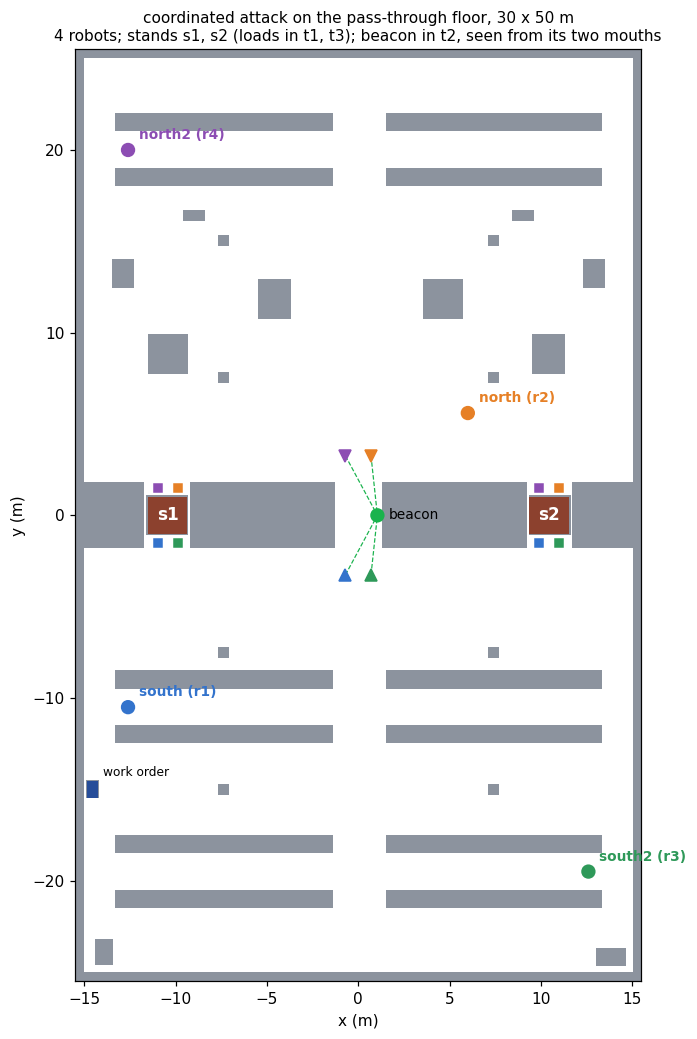
\includegraphics[width=0.5\textwidth]{figures/coordinated_attack_floor_n4.png}
\caption{The floor plan with four robots: south and south2 on the storage
floor, north and north2 on the dispatch floor, two viewpoints at each mouth of
$t_2$, and four corners under each load.}
\label{fig:floor}
\end{figure}

The floor generator checks the four geometric claims of the companion report
for every robot and every pair, by casting rays over the occupied cells of the
plan: no robot starts in sight of another or of the beacon; from its viewpoint
each robot sees the beacon; no robot under one end of a load sees one under the
other end; and every place a robot is sent is reachable over the inflated plan.
Two robots under the same end of a load see each other, which is the same side,
so meeting at the stand still gives no common knowledge over the four.

The performers are those of the companion report, made general. The signal
node checks that every robot the model places at a viewpoint has the beacon in
line of sight. The radio node puts the message on the receiver's inbox and
prints its content at any level, $\Kop{i}\Eop{G}^{\ell-1}\job(s)$. For
$\mathit{lift}$ every robot drives to its mouth of the stand, one start time is
fixed for all, each drives in under its corner along the line from its mouth,
and the load is raised.

%  ======================================================================
\section{Runs}
\label{sec:runs}

Both floors were run with four robots and two message levels, the order naming
$s_1$, and recorded on a $3840 \times 1080$ virtual display with RViz on the
left and Gazebo on the right. The beacon floor was also run with the order
naming $s_2$, without recording. In the tables the model column gives worlds
and designated worlds after the update, and the depth of mutual knowledge of
$\job(s_1)$ among the four.

\subsection{The radio floor}

\begin{table}[H]
\centering\small
\caption{The radio floor with four robots, as the run reported it.}
\label{tab:radio-run}
\begin{tabularx}{\textwidth}{@{}l X r@{}}
\toprule
action & reported & model \\
\midrule
plan & no policy for $\mathit{lifted}$ after 120.3\,s; cut off at depth 8 & 2 / 2 \\
$\mathit{read\text{-}order}$ & at the terminal after 16\,s; the order names $s_1$; $e_h$ & 2 / 1, $E^0$ \\
$\mathit{tell}(\ag{south}, \ag{north})$ & ``$\Kop{south}\job(s_1)$'' delivered & 4 / 1, $E^0$ \\
$\mathit{tell}(\ag{north}, \ag{south2})$ & ``$\Kop{north}\job(s_1)$'' delivered & 6 / 1, $E^0$ \\
$\mathit{tell}(\ag{south2}, \ag{north2})$ & ``$\Kop{south2}\job(s_1)$'' delivered & 8 / 1, $E^1$ \\
$\mathit{ack}(\ag{north2}, \ag{north})$ & ``$\Kop{north2}E\,\job(s_1)$'' delivered & 10 / 1, $E^1$ \\
$\mathit{ack}(\ag{north2}, \ag{south2})$ & delivered & 16 / 1, $E^1$ \\
$\mathit{ack}(\ag{north2}, \ag{south})$ & delivered & 34 / 1, $E^2$ \\
$\mathit{lift}(s_1)$ & knowledge requirement does not hold: \code{(C (south north south2 north2) job\_s1)} & refused \\
\bottomrule
\end{tabularx}
\end{table}

\noindent
On this floor the planner's 120\,s are a budget and not a proof: it was cut off
in the iteration at depth 8, and the mission then ran the protocol of
Table~\ref{tab:protocol}. The depths computed from the live model after each
message were those the replay computes offline, and the mission confirmed
through the epistemic state that $\Eop{G}^2\job(s_1)$ held among the four
robots and $\Cop{G}\job(s_1)$ did not. No robot moved toward a stand. The floor
runs to $\Eop{G}^2$, where the companion report's runs to $\Eop{G}^4$, because
the planner did not find the four-robot protocols for $\Eop{G}^3$ or
$\Eop{G}^4$ within its budgets.

\subsection{The beacon floor}

\begin{table}[H]
\centering\small
\caption{The beacon floor with four robots, as the run reported it.}
\label{tab:beacon-run}
\begin{tabularx}{\textwidth}{@{}l X r@{}}
\toprule
action & reported & model \\
\midrule
plan & 10 policy items, 2 leaves, 4.2\,s & 2 / 2 \\
$\mathit{go\text{-}view}(\ag{north})$ & at its viewpoint after 17\,s; beacon in line of sight, 3.3\,m & 2 / 2 \\
$\mathit{go\text{-}view}(\ag{south2})$ & at its viewpoint after 60\,s; 3.4\,m & 2 / 2 \\
$\mathit{go\text{-}view}(\ag{north2})$ & at its viewpoint after 62\,s; 3.9\,m & 2 / 2 \\
$\mathit{read\text{-}order}$ & at the terminal after 17\,s; the order names $s_1$; $e_h$ & 2 / 1, $E^0$ \\
$\mathit{go\text{-}view}(\ag{south})$ & at its viewpoint after 53\,s; 3.8\,m & 2 / 1, $E^0$ \\
$\mathit{signal}(\ag{south}, s_1)$ & in line of sight: all four, 3.3 to 3.8\,m & 3 / 1, $C$ \\
$\mathit{lift}(s_1)$ & at the mouths after 26 to 28\,s; joint start; under the load after 13.7 and 13.8\,s: starts 0.00\,s apart, arrivals 0.10\,s apart; load raised 0.12\,m, 50\,s after the lift began & 1 / 1, $C$ \\
\bottomrule
\end{tabularx}
\end{table}

\noindent
With the order naming $s_2$ the read gave $e_e$, the $s_2$ tier was lit with
all four robots in line of sight, $\Cop{G}\job(s_2)$ held, and the load on $s_2$
was raised with arrivals 0.70\,s apart.

\begin{figure}[H]
\centering
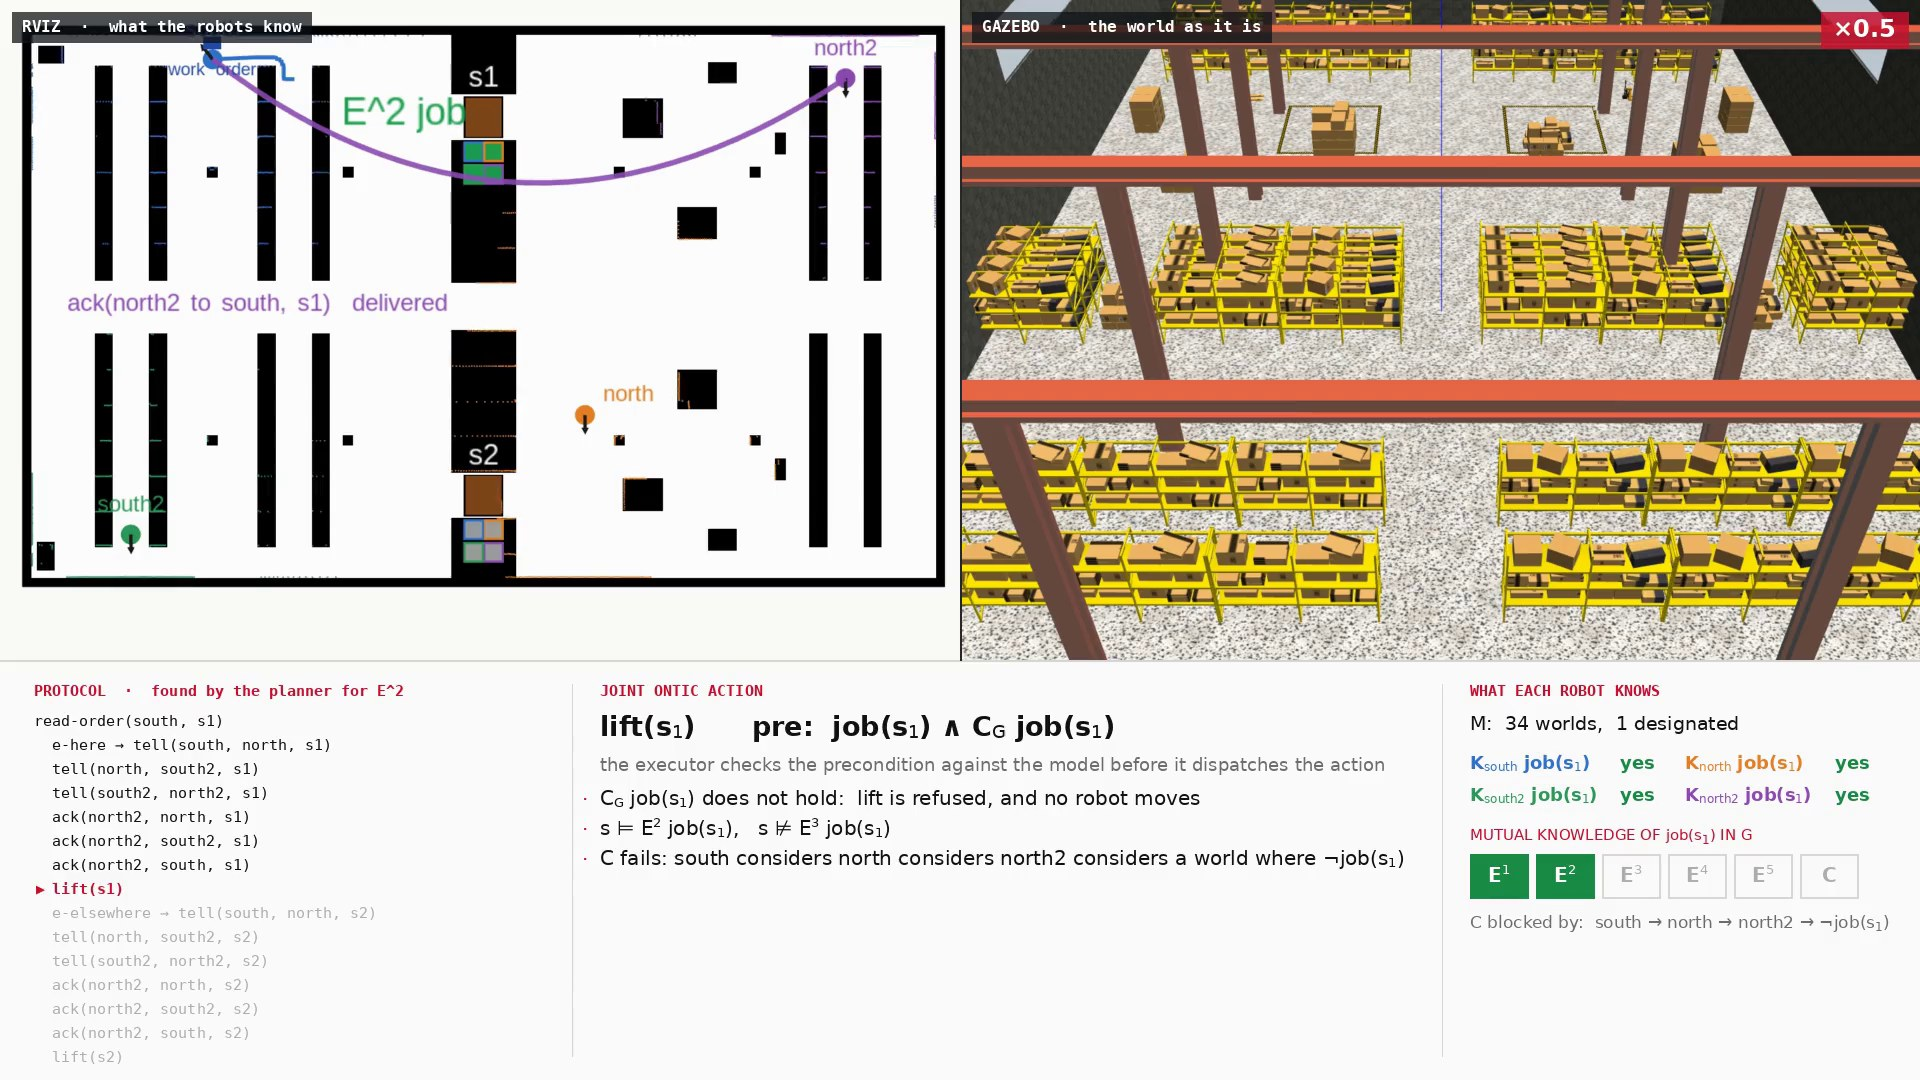
\includegraphics[width=\textwidth]{figures/coordinated_attack_scale_frame_refused.jpg}\\[0.4em]
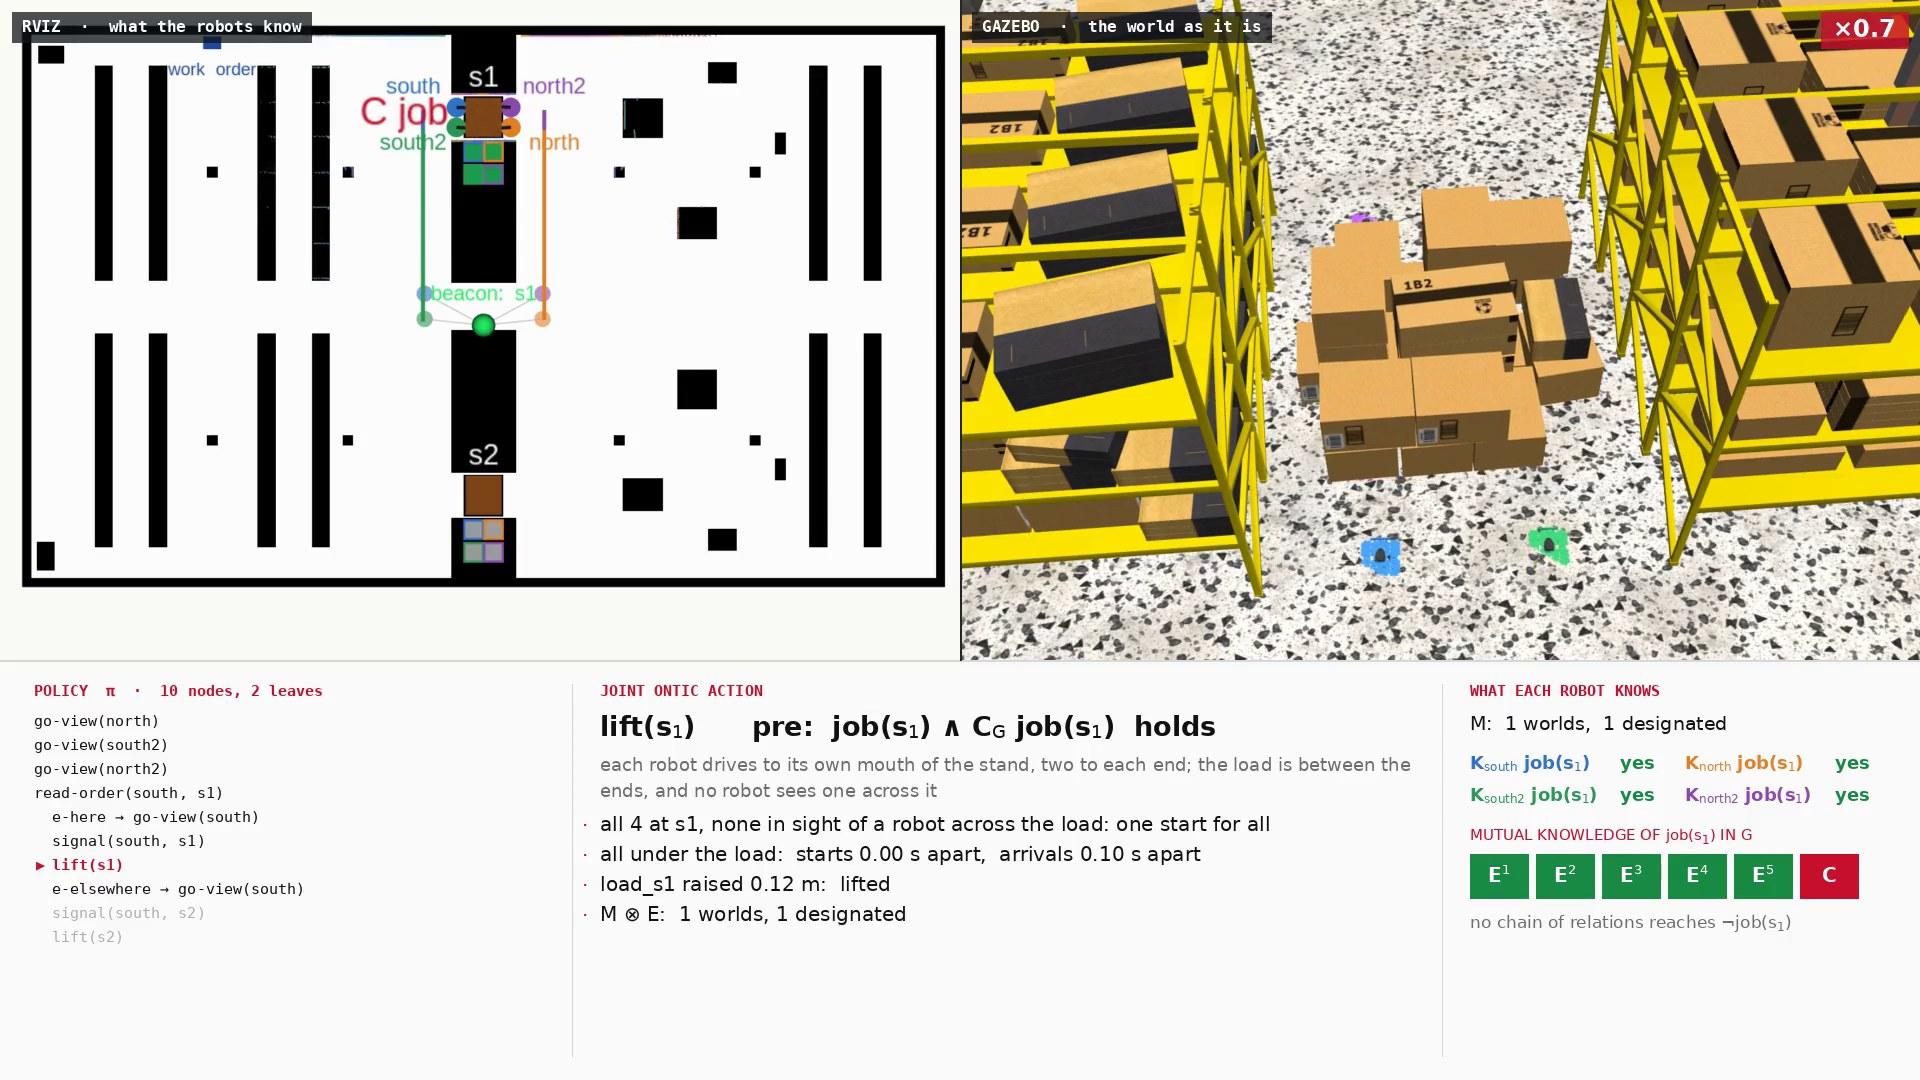
\includegraphics[width=\textwidth]{figures/coordinated_attack_scale_frame_lift.jpg}
\caption{Two frames of the film. Above, the radio floor after the sixth
message: 34 worlds, $E^2$ among the four robots, and the lift refused. Below,
the beacon floor during the lift, seen from above the bay: $C$, and the four
robots under the load.}
\label{fig:frames}
\end{figure}

%  ======================================================================
\section{Defects}
\label{sec:defects}

\paragraph{A base that drifts after turning} The first three four-robot runs of
the beacon floor, two with the order naming $s_1$ and one with $s_2$, lifted
with two robots short of the load and arrivals 11.4 to 11.6\,s apart. A
simulated Waffle that has turned on the spot and is then driven straight, with
an angular command of exactly zero, curves back toward the heading it arrived
on, by about 47 degrees over the metre and a half into the bay. A probe in an
isolated simulator reproduced it, and showed no drift without the prior turn.
The outer two robots ran into the side of the bay. The inner two drifted about
0.9\,m as well, and were counted as under the load only because the lift node
measured depth into the bay alone. The lift now creeps along the line from
each robot's mouth and steers back onto it, and the four arrive together. The
companion report's runs used the open-loop creep along the axis of the bay,
where a drift of that size still ends inside it; whether they drifted was not
measured, and neither was whether the other demonstrations that use the
open-loop creep are affected.

\paragraph{A client that stopped waiting} The first run of the four-robot radio
floor reported that the planner returned nothing after 15.0\,s. The planner was
still searching; the mission's planner client had waited its default of
15\,s. On the companion report's floors the planner answers in under a second,
while on the four-robot radio floor it searches its whole budget, and the
client is now given that budget and fifteen seconds more.

\paragraph{A count of levels that was not the model} The first version of the
ladder tool counted only the highest level each robot had heard from each
other, and searched over that count. Random sequences replayed through the
product update refuted it: after $\mathit{tell}(\ag{south},\ag{north})$,
$\mathit{tell}(\ag{north},\ag{south})$ and $\mathit{ack}(\ag{south},\ag{north})$
the depth is $E^3$, where the count gave $E^2$. The count missed what a message
says beyond its content, and the ladder is now searched by the planner over the
domain itself.

\paragraph{The simulator at start} gzserver crashed at startup in one run and in
one probe, while the second robot's plugins loaded and before the third was
spawned. The run was repeated unchanged.

%  ======================================================================
\section{What the runs establish}
\label{sec:established}

That the companion report's account of the coordinated attack does not depend
on there being two robots. With a type for the robots that neither send nor
receive a message, the bound of one level per message holds for any group, and
the radio floor has no policy for any number of robots or messages; one signal
from viewpoints that are common knowledge yields common knowledge over all of
them.

That the account holds on the floor with four robots: six delivered messages
among them gave $E^2$, computed from the live model after each message as the
replay computed it offline, and the executor refused the lift; one signal gave
common knowledge over all four, and the four lifted together.

And that what scale changes is the cost. Replanning finds the beacon policy for
ten robots in under a second, while the proofs on the radio floor run out of
budget from three robots and two levels; and among $N$ robots each level of
mutual knowledge cost $N-1$ messages in every cell the planner settled, because
a message carries what it implies about who could have sent it.

%  ======================================================================
\section{Directions for the next iteration}
\label{sec:next}

\paragraph{The cost of a level} Among $N$ robots, $E^k$ cost $k(N-1)$ messages
in every cell the planner settled, and in the cells it did not settle it showed
that fewer do not suffice. For two robots the count is
Proposition~\ref{prop:onelevel}. Whether it holds for every $N$ is open, and
needs an argument, since no finite set of cells settles it.

\paragraph{Positions with more robots} The sighting and the unconfirmed
announcement of the companion report are written for a pair, and a version for
a group of robots was not attempted.

\paragraph{Larger floors} The floor has places for four robots. More would need
viewpoints of the beacon and corners under the loads for each, and the planner
reaches the beacon policy by replanning for ten.

%  ======================================================================
\begin{thebibliography}{9}
\bibitem{akkoyunlu1975} E.~A. Akkoyunlu, K.~Ekanadham and R.~V. Huber.
  Some constraints and tradeoffs in the design of network communications.
  In \emph{Proceedings of the 5th ACM Symposium on Operating Systems
  Principles}, pages 67--74, 1975.
\bibitem{fhmv1995} R.~Fagin, J.~Y. Halpern, Y.~Moses and M.~Y. Vardi.
  \emph{Reasoning About Knowledge}. MIT Press, 1995.
\bibitem{gray1978} J.~Gray.
  Notes on data base operating systems.
  In \emph{Operating Systems: An Advanced Course}, LNCS 60, pages 393--481.
  Springer, 1978.
\bibitem{halpern1990} J.~Y. Halpern and Y.~Moses.
  Knowledge and common knowledge in a distributed environment.
  \emph{Journal of the ACM}, 37(3):549--587, 1990.
\bibitem{ulises2026ca} H.~Ulises.
  The coordinated attack on a warehouse floor: common knowledge as an action
  precondition, a lossy channel that cannot supply it, and a signal that can.
  Epistemic Robotics report, 2026.
\bibitem{vanditmarsch2007} H.~van Ditmarsch, W.~van der Hoek and B.~Kooi.
  \emph{Dynamic Epistemic Logic}. Springer, 2007.
\end{thebibliography}

%  ======================================================================
\section*{Reproduction}

\begin{lstlisting}
ros2 launch coordinated_attack_demo coordinated_attack_launch.py robots:=4 messages:=2
ros2 launch coordinated_attack_demo coordinated_attack_launch.py robots:=4 messages:=2 order:=s2
ros2 launch coordinated_attack_demo coordinated_attack_launch.py robots:=4 messages:=2 floor:=radio
bash tools/validate.sh                                   # thirteen checks, no simulator
python3 tools/scaling.py --out /tmp/ca_scaling           # the two planning tables
python3 tools/ladder.py --table 2,3,4,5 --depths 1,2,3,4,5 --out /tmp/ca_ladder
python3 tools/ladder.py --replay protocols/radio-n4-m2.json --out /tmp/ca_replay
ROBOTS=4 MESSAGES=2 bash tools/record_demo.sh beacon s1 /tmp/raw_n4.mkv  /tmp/run_n4.log
ROBOTS=4 MESSAGES=2 bash tools/record_demo.sh radio  s1 /tmp/raw_n4r.mkv /tmp/run_n4r.log
\end{lstlisting}

\end{document}
